\chapter{Inference}
Firstly we want to study the correlation between various features we have studies above. But before that we need to do data scaling. It may be carried out in 2 options : 1) \textbf{Normalization} 2) \textbf{Standardization}. As most of the algorithms assume the data to be normally (Gaussian) distributed, \textbf{Normalization} is done for features whose data does not display normal distribution and \textbf{standardization} is carried out for features that are normally distributed where their values are huge or very small as compared to other features.
\begin{itemize}
    \item \textbf{Oldpeak} feature is normalized as it had displayed a right skewed data distribution.
    \item  \textbf{Age}, \textbf{RestingBP}, \textbf{Cholesterol} and \textbf{MaxHR} features are scaled down because these features are normally distributed.
\end{itemize}

\section{Correlation matrix}
\begin{figure}[!htpb]
    \centering
    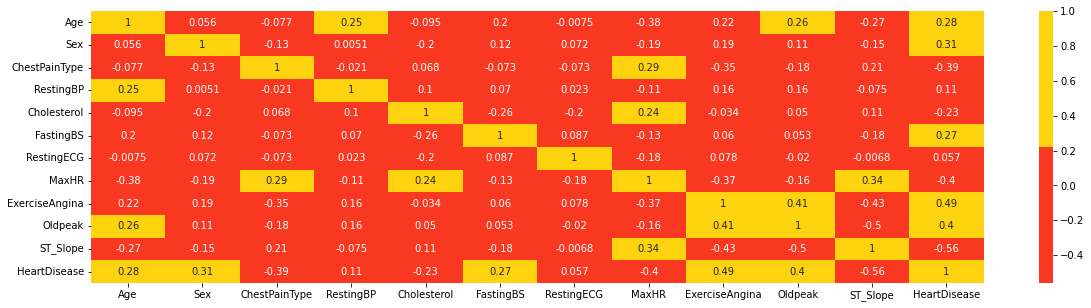
\includegraphics[width=\linewidth]{Figures/Outputs/corr-mat.png}
    \label{Correlation matrix}
    \caption{The correlation matrix between various features.}
\end{figure}

As we may observe, it is a huge matrix with too many features. We only want to look at correlation against heart diseases.
\begin{figure}[!htpb]
    \centering
    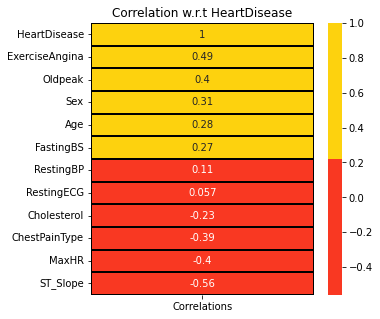
\includegraphics[width=0.7\linewidth]{Figures/Outputs/corr-hd.png}
    \label{Correlation between features and heart disease.}
    \caption{Correlation between features and heart disease.}
\end{figure}

Except for \textbf{RestingBP} and \textbf{RestingECG}, everyone displays a positive or negative relationship with \textbf{HeartDisease}.

\section{$\chi^2$-test for categorical features}
\begin{figure}[!htpb]
    \centering
    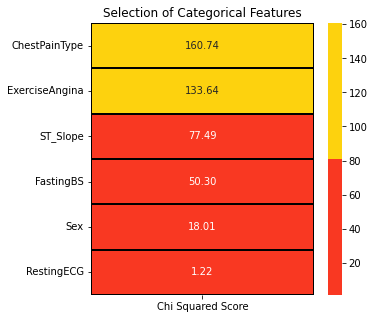
\includegraphics[width=0.6\linewidth]{Figures/Outputs/chi-sq.png}
    \label{Chi-squared scores for various features}
    \caption{$\chi^2$-scores for the categorical features.}
\end{figure}

Except \textbf{RestingECG}, all the remaining categorical features are pretty important for predicting heart diseases.

\section{ANOVA test for numerical features}
\begin{figure}[!htpb]
    \centering
    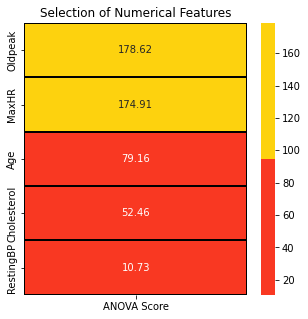
\includegraphics[width=0.6\linewidth]{Figures/Outputs/anova.png}
    \label{ANOVA for numerical features}
    \caption{ANOVA-scores for numerical features}
\end{figure}

\textbf{RestingBP doesn't seem as influential as the remaining features.}